\subsection{Teleporation in spherical space} \label{sub:teleportation}
Even though splitting the scene into two regions in spherical geometry allows us to minimize distortions significantly, it introduces a wide range of other problems.
The most important one has to do with moving objects and the camera from one region to the other; we call this process \textit{teleportation}.

Teleportation is schematically shown in \autoref{fig:teleportation}.
\begin{figure}[h]
    \centering
    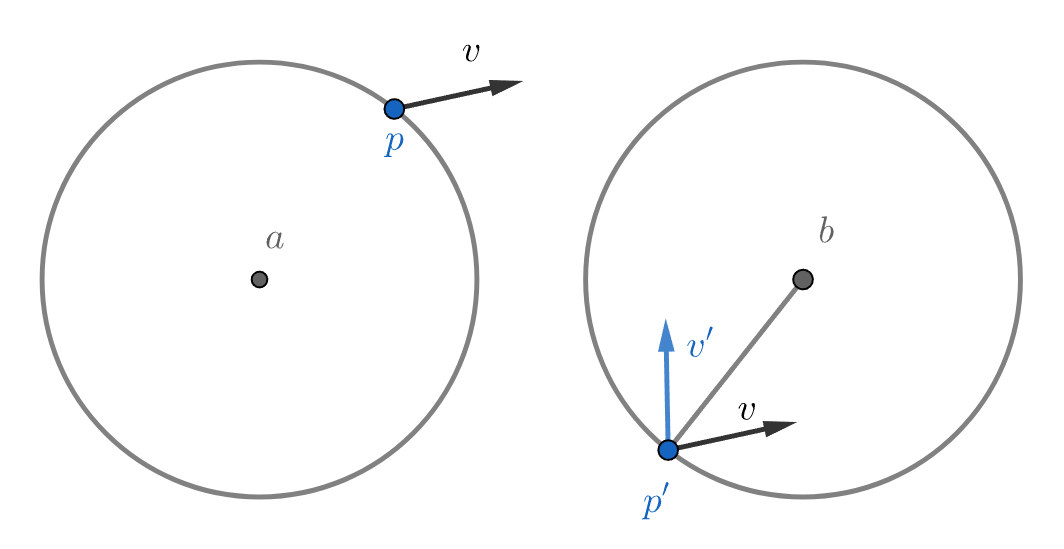
\includegraphics[width=0.6\textwidth]{chapters/theoretical_foundations/sections/non-eudlidean-spaces/resources/teleportation.png}
    \caption{Teleportation between two regions}
    \label{fig:teleportation}
\end{figure}
In this 2-dimensional example, an object leaves the first region (centered at $a$) at the point $p$ and is teleported to the second region (centered at $b$), appearing at a location given by the point $p'$:
\begin{equation*}
    p' = b + R_{xz}(p - a),
\end{equation*}
where $R_{xz}(p)$ denotes reflection of a point $p$ across the origin.
The velocity vector $v$ of the object is mapped to vector $v'$ which is the reflection of $v$ on a vector $p - a$.

The teleportation in the 3-dimensional case can be defined in a very similar manner.
There are only two differences.
The first one is that $R_{xz}(p)$ now denotes a reflection on the unit vector $\hat{y}$ (assuming positive $y$ direction coincides with the "up" direction for the scene).
The second difference is that $v'$ is now the reflection of $v$ through a plane through the origin orthogonal to $(p - a) \times \hat{y}$.

To account for the point reflection $R_{xz}$, the porting given by \autoref{eq:spherical-port-2} has to be modified by replacing $p'$ with $R_{xz}(p')$.

Setting up the view transformation in the second region also comes with its own set of challenges.
The standard way of obtaining the vectors $i'$, $j'$, and $k'$ for the view matrix \ref{eq:view-matrix} is as follows.
We first port the camera position to non-Euclidean space (in the case of the second region, we use \autoref{eq:spherical-port-2}), and then use the \autoref{eq:porting-vector} to port its right, up, and front vectors.
The problem with this approach is that the translation matrix \ref{eq:translation-matrix} is defined in terms of translating the geometry origin $g = (0, 0, 0, 1)$ and not $(0, 0, 0, -1)$.
This means that if the translation target $q$ is close to $(0, 0, 0, -1)$, $T(q)$ can map a point $p$ with $p_w < 0$ to a new point $p'$ with $p'_w > 0$ because
\begin{equation*}
    p'_w = -q_x p_x - q_y p_y - q_z p_z + q_w p_w \approx q_w p_w > 0.
\end{equation*}
The matrix isn't even defined for translation targets with $q_w = -1$.

To solve this problem, we derived a translation matrix $T_2(q)$ which we use for translations in the second region.
It is defined analogously to $T(q)$ given by \autoref{eq:translation-matrix}, but in the context of $T_2$, the translation target $q$ is the point that the point $(0, 0, 0, -1)$ is translated to.
The matrix is given by
\begin{equation}
    T_2(q) = \begin{bmatrix}
        1 - \frac{q_x^2}{1 - q_w} & -\frac{q_x q_y}{1 - q_w}  & -\frac{q_x q_z}{1 - q_w}  & q_x  \\
        -\frac{q_y q_x}{1 - q_w}  & 1 - \frac{q_y^2}{1 - q_w} & -\frac{q_y q_z}{1 - q_w}  & q_y  \\
        -\frac{q_z q_x}{1 - q_w}  & -\frac{q_z q_y}{1 - q_w}  & 1 - \frac{q_z^2}{1 - q_w} & q_z  \\
        -q_x                      & -q_y                      & -q_z                      & -q_w
    \end{bmatrix}.
\end{equation}
Using the fact that $q$ is in the spherical geometry, i.e. $\langle q, q \rangle_E = 1$, it can be verified that the row vectors of the matrix are orthonormal, thus the matrix describes an isometry.
Moreover, $T_2((0, 0, 0, -1))$ is the identity matrix as expected.